\documentclass[a4paper]{article}
\usepackage{geometry}
\geometry{a4paper, portrait, margin=1in}
\usepackage[english]{babel}
\usepackage[utf8]{inputenc}
\usepackage{natbib}
\usepackage{graphicx}
\usepackage{fancyhdr}
\usepackage{array}
\usepackage{tabu}
\usepackage{listings}
\usepackage[export]{adjustbox}
\graphicspath{{/Users/ThomasBass/GitHub/GSCE-Coursework-Weblang-TrafficLights/Images/}}
\DeclareGraphicsExtensions{.png}




\title{Computing GCSE Coursework}
\author{\\ \\ \\ \\ Thomas Bass\\Candidate 4869\\Centre 52423\\OCR A452 Practical Investication\\\\Word Count: 915\\\\Made with \LaTeX}
\date{2017}


\pagestyle{fancy}
\fancyhf{}
\rhead{Computing GCSE Coursework}
\chead{Candidate 4869}
\lhead{Thomas Bass}
\rfoot{Page \thepage}

\begin{document}

\maketitle
\pagebreak
\renewcommand*\contentsname{Summary}
\tableofcontents
\pagebreak

%%%%%%%%%%%%%%%%%%%%%%%%%%%%%%%%%%%%%%%%%%%%%%%%%%%%%%%%%%%%%%%%%%%%%%%%%

\section{Task 1}
Often, a web designer wants a change to happen when a user clicks on a screen object or moves the mouse over it. JavaScript can make changes to the HTML elements. \par
\noindent Enter and run this script: \par \par
\begin{lstlisting}
<!DOCTYPE html>
<html>
<body>
<h1>Change an HTML element</h1>
<p id="msg">Now you see me.</p>
<button type="button"
onclick="document.getElementById('msg').innerHTML = 'Gone!'">
Click Me!</button>
<button type="button"
onclick="document.getElementById('msg').innerHTML = 'Back again!'">
Bring me back!</button>
</body>
</html>
\end{lstlisting}
	

\subsection{Explain how you ran this script:} ~\par	

This script was copied into a HTML document, and opened into a web browser. 

When the script ran it gave the following output: ~\par ~\par
\noindent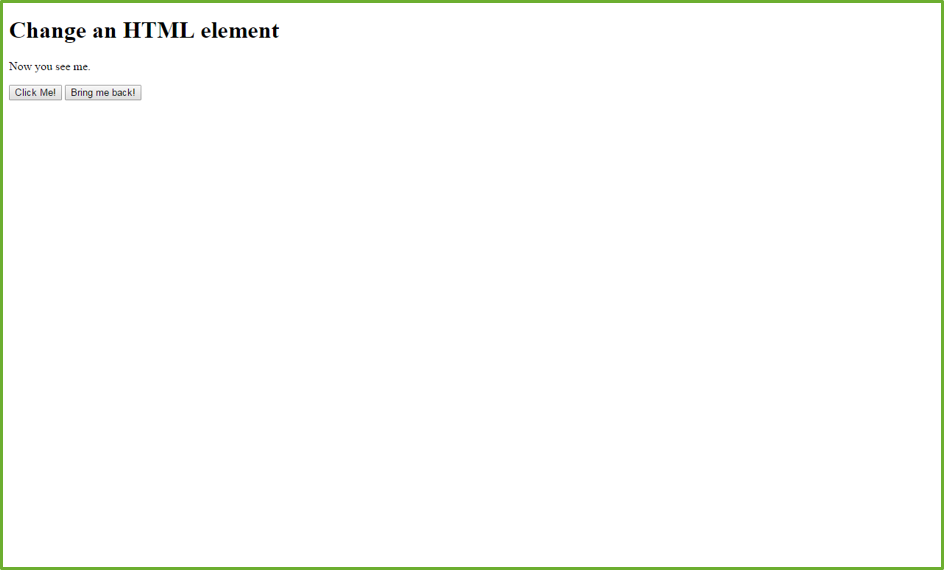
\includegraphics[width=0.5\textwidth, left, width=\linewidth, frame]{Picture1.png}

The web page took the code entered, ran it, and produced this output.
\newpage
\subsection{Explain what each line of the script does:}
\subsubsection{The HTML Code:}
\begin{lstlisting}
01	<!DOCTYPE html>
02	<html>
03	<body>
04	<h1>Change an HTML element</h1>
05	<p id="msg">Now you see me.</p>
06	<button type="button"
07	onclick="document.getElementById('msg').innerHTML = 'Gone!'">
08	Click Me!</button>
09	<button type="button"
10	onclick="document.getElementById('msg').innerHTML = 'Back again!'">
11	Bring me back!</button>
12	</body>
13	</html>
\end{lstlisting}
\subsubsection{Commentry:}

\begin{lstlisting}
01	This declares that the document is a HTML document
02	This opens the <html> tag, and shows that the code enclosed 
	is HTML code
03	This opens the <body> tag, and shows that the code enclosed 
	is placed in the body of the document
04	This opens the <h1> tag, showing that the text enclosed 
	("Change an HTML Element") is placed in the highest header, and closes
	the tag
05	This opens a <p> tag, showing that the text enclosed ("Now you see me.")
	is paragraph text, and it has the ID "msg", and then the tag is closed
06	This opens a <button> tag, showing that the information enclosed is 
	a button, and has type "button"
07	This declares that following an onclick event (when the button is clicked),
	the program will execute a Javascript function to find the elements with 
	the ID of "msg" (the body text in line 05) and change its HTML code to "Gone".
08	This line provides the text of the button ("Click Me!") and closes the 
	<button> tag
09	This opens a <button> tag, showing that the information enclosed is 
	a button, and has type "button"
10	This declares that following an onclick event (when the button is clicked),
	the program will execute a Javascript function to find the elements with 
	the ID of "msg" (the body text in line 05) and change its 
	HTML code to "Back Again!".
11	This line provides the text of the button ("Bring me back!") and closes the 
	<button> tag
12	This closes the <body> tag
13	This closes the <body> tag and ends the document
\end{lstlisting}
\newpage
%%%%%%%%%%%%%%%%%%%%%%%%%%%%%%%%%%%%%%%%%%%%%%%%%%%%%%%%%%%%%%%%%%%%%%%%%
\section{Task 2}
As is the case with most programming languages, in JavaScript you can use arrays in order to store multiple values under the same identifier. For example, an array of products can be set up as below for use on an ecommerce web site.\par
  \verb|var products = ["Printer","Tablet","Router"];|

\subsection{Set up an array to include the items shown above, plus a few extras of your choice.}
\subsubsection{Products:}
Printer, Tablet, Router, Network Switch, Monitor, Keyboard, Mouse, 500GB Hard Drive, ATX Motherboard, Memory Card, Flash Drive, Network Switch, Bluetooth Adaptor, Modem, Wireless Speaker, 256GB SSD.
\subsubsection{Array:} 
\begin{lstlisting}
var products = ["Printer","Tablet","Router","Network Switch","Monitor",
"Keyboard","Mouse","500GB Hard Drive","ATX Motherboard","Memory Card",
"Flash Drive","Network Switch","Bluetooth Adaptor","Modem",
"Wireless Speaker", "256GB SSD"];
\end{lstlisting}
=16 items

\subsubsection{Array in code editor:}
\noindent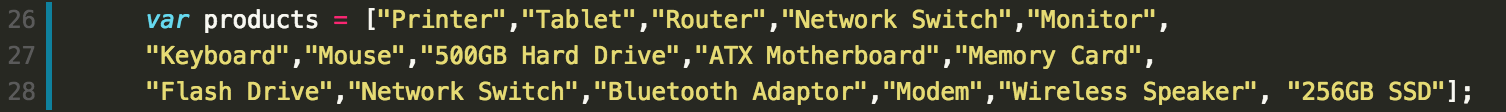
\includegraphics[width=1\textwidth, left, width=\linewidth, frame]{Picture2.png}

\subsection{Write a script that:}
\subsubsection{Outputs the items in alphabetical order}
\noindent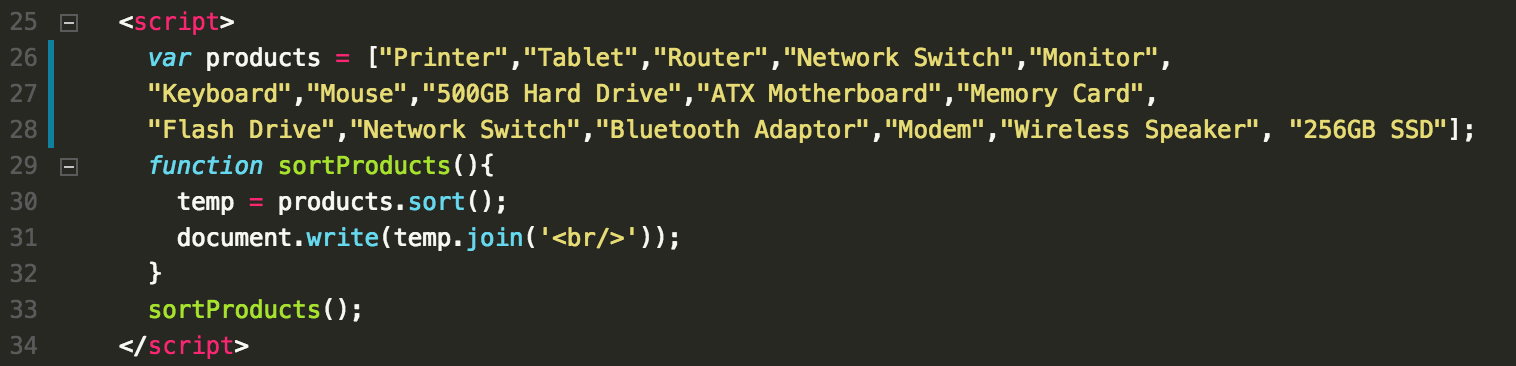
\includegraphics[width=1\textwidth, left, width=\linewidth, frame]{Picture3.png} \par
This code snippet is written in JS embedded in an HTML document. Line 25 opens the \verb|<script>| tag, which indicates to the HTML code that the following is JS script. Lines 26 to 28 then declares \verb|products| to be a global array with the contents as described in part 2.1. Line 29 declares \verb|sortProducts()| to be a function, and opens the code for the function. Line 30 declares \verb|temp| to be the array \verb|products|, sorted alphabetically with the \verb|.sort| function built into JS. Line 31 then outputs the \verb|temp| array, joined by a \verb|<br>| line break, onto the document body with the \verb|.write| function. Line 32 closes the code for the \verb|sortProducts()| function, and Line 33 calls the \verb|sortProducts()| function its self. Line 34 then closes the \verb|<script>| tag, indicating the end of this JS script. \newpage
\subsubsection{Counts the number of items in the array.}
\noindent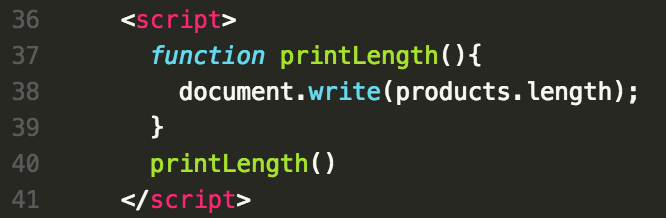
\includegraphics[width=0.4\textwidth, left]{Picture4.png} \par
This code snippet is again written in JS, and embedded in the same HTML document as in 2.2.1. Line 36 opens the \verb|script| tag to declare the following as JS code. Line 37 then declares \verb|printLength()| to be a function, and opens the code for the function. Line 38 outputs the length of the array with the built-in \verb|.length| function, and writes it to the body with \verb|.write|.  The code is then closed in line 39, and the \verb|printLength()| function is called in line 40. Line 41 then closes the \verb|<script>| tag to show the end of the JS script.
\subsubsection{Full code:}
\noindent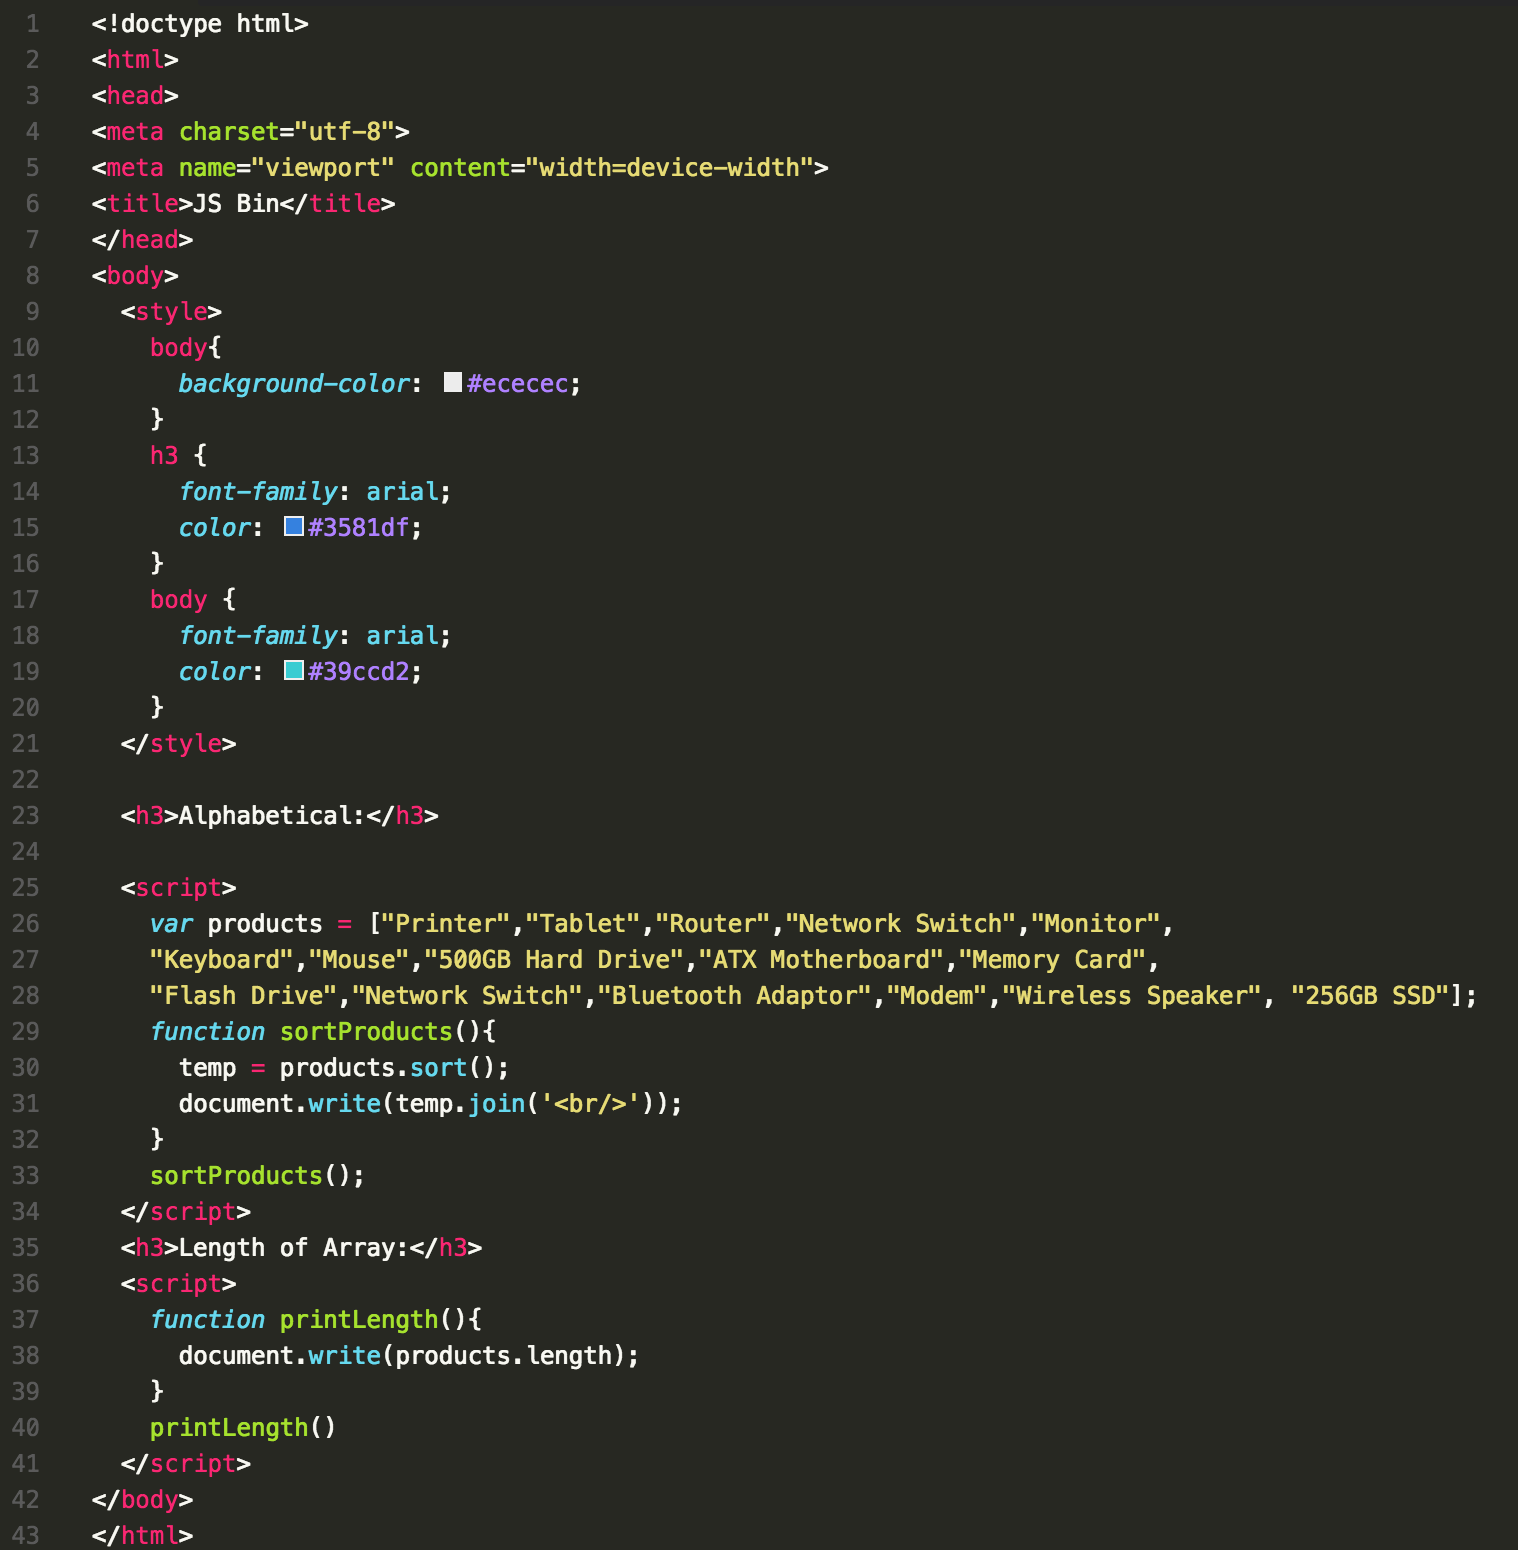
\includegraphics[width=1\textwidth, left, width=\linewidth, frame]{Picture5.png} \par \newpage
\subsubsection{Output:}
\noindent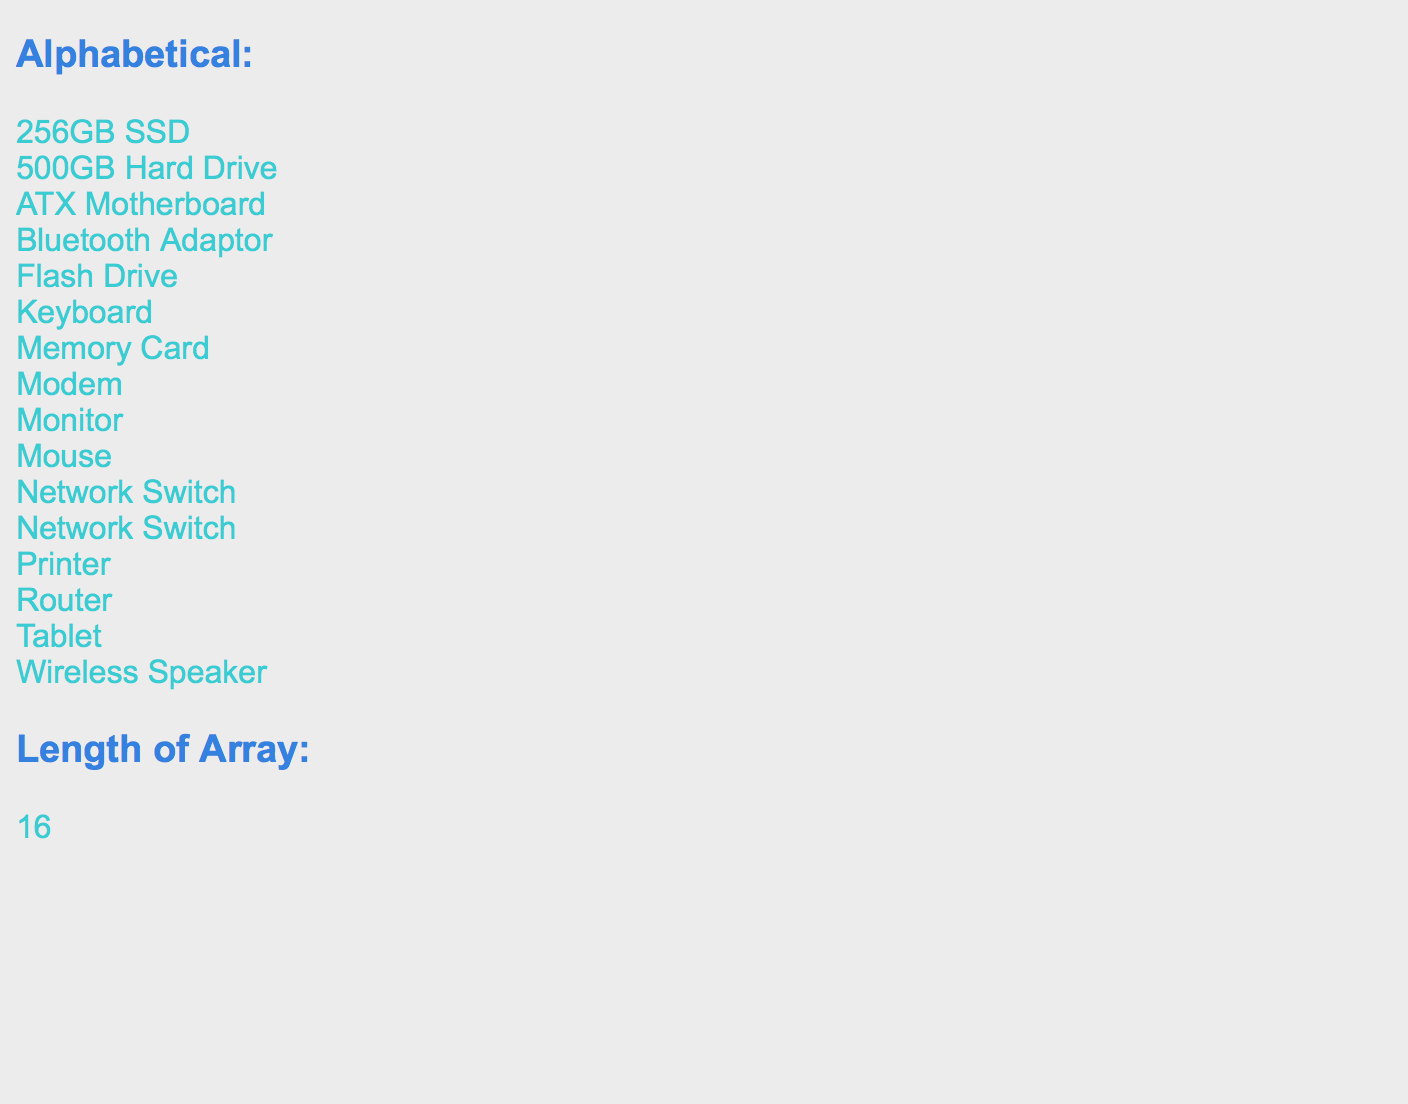
\includegraphics[width=1\textwidth, left, width=\linewidth, frame]{Picture6.png} \par \newpage

\section{Task 3}
\subsection{(i) Make a list of assets that will be required in order to produce this display.}
\begin{center}
\begin{tabular}{ | m{9em} | m{10em} | m{15em} | m{8em} | }
  \hline
  Asset Name & Asset Type & Asset Description & Asset Properties	\\ [0.5ex] 
  \hline \hline	
  Traffic light frame & FlexBox Container & The frame for the traffic lights & Black with White border \\
  \hline
  Red traffic light & FlexBox Item & The red traffic light & Dimmed Red (\#49180d) \\
  \hline
  Amber traffic light & FlexBox Item & The amber traffic light & Dimmed Amber (\#8f7414) \\
	\hline
	Green traffic light & FlexBox Item & The green traffic light & Dimmed Green (\#0d4913) \\
	\hline
	Traffic Light Label & Button & A label for the traffic light, and to help FlexBox spacing & No OnClick event, grey \\
	\hline
	Wait signal box & FlexBox Container & The frame for the pedestrian wait button & Black \\
	\hline
	Wait signal button & Button & The button to stop the lights for a pedestrian & Black \\
	\hline
	Interval change container & FlexBox Container & The container for the interval change button and text & Invisible \\
	\hline
	Interval change button & Button & Button to call the interval time change dialogue box & \#1fadcf \\
	\hline
\end{tabular}
\end{center}
\subsection{(ii) Describe and explain where the assets will be best located.}
For this task, as it is a small, single page website, all the scripts and styles will be embedded into the HTML document. The objects will be arranged in \verb|<div>| structures, and items will be inside FlexBoxes.
FlexBoxes are a CSS Layout style, where flexible boxes contain items. This means that the objects are dynamically aligned, and no positioning is fixed or absolute. This makes it usable on mobile devices as well as a range of screen sizes. It is also adaptable, and easy to adjust. My reaserch primerially came from the W3Schools page on FlexBoxes: http://www.w3schools.com/css/css3_flexbox.asp

\section{Task 4}

%%%%%%%%%%%%%%%%%%%%%%%%%%%%%%%%%%%%%%%%%%%%%%%%%%%%%%%%%%%%%%%%%%%%%%%%
\section{Task 5}
Scripts can be embedded in the HTML of web pages or saved externally as script files. Discuss the benefits and drawbacks of each approach.
\subsection{Embedded JS Scripts}
JavaScript functions can easily be embedded into an HTML document, like I've done in tasks 3 and 4. In HTML, the \verb|<script>| tag opens the area for JS code, but must be closed afterwards. For example, a button can have the \verb|onclick()| event for \verb|change()|, which will call the \verb|change()| function in the JavaScript area. For a demo, I used jsbin.com, a website where you can write and run HTML, JS and CSS code embedded or in a separate area. I entered the following demo code: \par
\noindent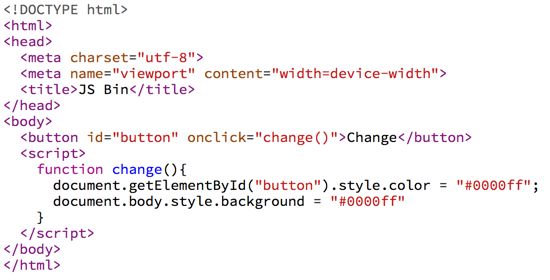
\includegraphics[width=0.7\textwidth, left, width=\linewidth, frame]{Picture7.png}
On the click of the button with id of \verb|button|, the \verb|change()| function will be called from the \verb|<script>| area. The function changes the color of the element with ID of \verb|button| to blue and changes the body background to blue. The first lines inside the \verb|<head>| tag and with the \verb|<meta>| tags is just information about the document and is irrelevant to the task. This was the output before the button was clicked: \par
\noindent
\includegraphics[width=1\textwidth, left, width=\linewidth, frame]{Picture8.png}\par \newpage
And this was the output after the button was clicked: \par
\noindent
\includegraphics[width=1\textwidth, left, width=\linewidth, frame]{Picture9.png}
This clearly show that the embedded script can easily change the style of HTML elements. This could be adapted to change position, size, and any other attribute. \newpage
\subsection{External JS Scripts}
The same effect as in 3.1 can be made with externally saved scripts. Alongside the HTML file (normally named \verb|index.html|) the JS file can be saved (normally named \verb|script.js|. In this scenario, the CSS styling is also saved externally, rather than embedded as the \verb|<style>| tag, normally as \verb|style.css|. I adapted the demo code in 3.1 to show this. \par
\noindent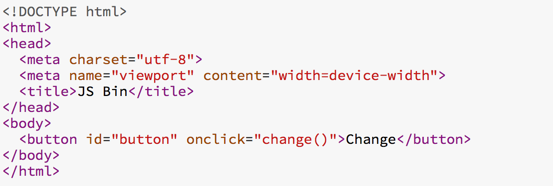
\includegraphics[width=0.7\textwidth, left, width=\linewidth, frame]{Picture10.png}
This is the HTML code, which is the same as before in 3.1, but with the \verb|<script>| code removed. This document is now entirely HTML. The JS was moved to the external file: \par
\noindent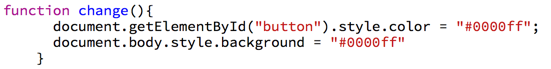
\includegraphics[width=0.7\textwidth, left, width=\linewidth, frame]{Picture11.png}
This shows the \verb|change()| function moved to the external file. This program will operate in the exact same way, as the files are both saved in the same location. Here is the output before the button was clicked: \par
\noindent
\includegraphics[width=1\textwidth, left, width=\linewidth, frame]{Picture12.png} 
And this is the output after the button was clicked: \par
\noindent
\includegraphics[width=1\textwidth, left, width=\linewidth, frame]{Picture13.png} 
As you can see, this produces the exact same results. So what are the benefits and drawbacks of each approach? \par \par
The embedded script approach is more suitable to small projects, such as a personal portfolio or small website. Having it all saved to the same file can make it a lot easier to manage, as well as preserving consistency and ensuring no failures. However, for larger tasks like a web app or large website, external scripts are often more applicable. \par
With an external script, pre-made code can be referenced from the HTML document and used elsewhere. This limits the size of the HTML document and makes it a lot tidier and easier to have consistent indentation. Websites like www.dynamicdrive.com offer scripts for both JS and CSS that can be embedded into the code easily. These off-the-shelf snippets are useful in small-scale webpages and can be embedded or saved externally, but are normally embedded. \par
I prefer to use embedded scripts, as I often code small-scale projects and it is easier to have it all in the same document. However, if a project gets to large, I will move my JS and CSS to an external file for consistency, and to reduce the time it takes for a page to load.





\end{document}